% -*- root: ../../../main.tex -*-
\subsection{Configuration Changes}
La configurazione del sistema può cambiare nel tempo, ad esempio quando una macchina va incontro a crash, viene sostituita o viene aggiunta al cluster.\\

Le informazioni sulla configurazione del sistema sono cruciali perchè sapere \textbf{quanti} e \textbf{quali} server fanno parte del cluster è necessario per operazioni che necessitano di decidere basandosi sulla maggioranza, come l'elezione del leader o il commit di una entry.\\

\subsubsection{Contemporanea presenza di due configurazioni}
  Il problema che si incontra in tutti i sistemi distribuiti è che \textit{la \textbf{transizione} tra una configurazione e l'altra \textbf{non avviene nello stesso istante} per tutte le macchine}. Esisterà dunque un tempo \textbf{t} per cui \textbf{alcune} macchine saranno aggiornate sulla \textbf{nuova configurazione} mentre \textbf{altre} saranno ancora nella \textbf{vecchia}. Ciò porta a una situazione in cui è possibile che ci siano due gruppi di server, che si trovano in \textbf{due diverse configurazioni} e che rappresentano la \textbf{maggioranza} per quella configurazione.\\

  \begin{figure}[H]
    \centering
    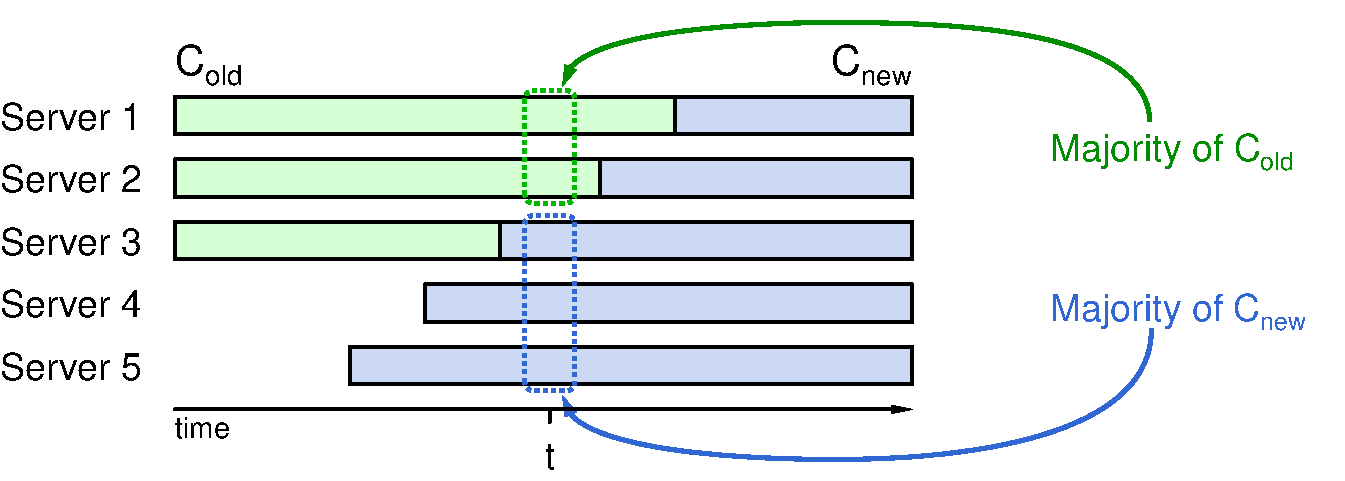
\includegraphics[width=0.90\columnwidth]{raft/configChanges.pdf}
    \caption{Esempio di \textbf{maggioranze diverse in due diverse configurazioni}: i server \textit{S4} e \textit{S5} entrano a far parte del cluster, ma al tempo \textbf{t}, si ha che \textit{S1} e \textit{S2} sono ancora alla \textbf{vecchia configurazione}, mentre \textit{S3}, \textit{S4} e \textit{S5} sono \textbf{passati alla nuova}.
    \textit{S1} e \textit{S2} costituiscono una maggioranza, nella configurazione vecchia (sono \textbf{2 su 3}), ma anche \textit{S3}, \textit{S4} e \textit{S5} possono formare una maggioranza nella loro configurazione di riferimento (\textbf{3 su 5}). }
    \label{fig:figure 8}
  \end{figure}

  \subsubsection{Problema}
    Sulla base di queste \textbf{maggioranze} possono essere portate a termine delle operazioni, come ad esempio, il commit  di una entry. Questo potrebbe generare delle \textbf{inconsistenze}, come nel caso seguente:
  \begin{enumerate}
    \item{\emph{I server \textbf{S1} e \textbf{S2} formano una \textbf{maggioranza} nella \textbf{vecchia} configurazione}}
    \item{\emph{I server \textbf{S3}, \textbf{S4} e \textbf{S5} formano una \textbf{maggioranza} nella \textbf{nuova} configurazione}}
    \item{\emph{la \textbf{maggioranza} data da S1 e S2 decide di fare \textbf{commit} dell'entry \textbf{e1}}}
    \item{\emph{la \textbf{maggioranza} data da S3,S4 e S5 decide di fare \textbf{commit} dell'entry \textbf{e2!=e1}}}
    \item{\emph{in corrispondenza dello \textbf{stesso indice}, si avranno dei \textbf{log diversi} che porteranno all'esecuzione di istruzioni diverse, generando \textbf{inconsistenza}}}
  \end{enumerate}

  Per risolvere questo problema, il passaggio tra una configurazione e l'altra non è immediato, ma viene fatto in \textbf{due fasi}.
    


  \subsubsection{Soluzione}   

    Per cambiare la configurazione del sistema, si ricorre a una \textbf{fase intermedia} posta tra la vecchia configurazione e quella nuova, in maniera tale da \textbf{evitare} di incorrere in \textbf{inconsistenze}.
    Durante questa fase intermedia, chiamata \textbf{joint consensus}, per prendere le decisioni si tengono in considerazione entrambe le maggioranze: sia quella della nuova configurazione (\textit{C\_new}) che quella della vecchia (\textit{C\_old}) in maniera tale che nè \textit{C\_old} nè \textit{C\_new} possano prendere \textbf{decisioni unilaterali}.\\

    Le caratteristiche di questo approccio sono le seguenti:
    
    \begin{itemize}
      \item{\textbf{Cambiamento della configurazione:} il passaggio a una nuova configurazione viene innescato da una richiesta. Quando il leader riceve questa richiesta la aggiunge al proprio log e la propaga, come farebbe normalmente, ma l'azione ha \textbf{effetto immediato} poichè il leader applica il cambiamento di configurazione il prima possibile, \textbf{senza attendere il commit}.}

      \item{\textbf{Configurazione intermedia:} successivamente, il leader, passa alla configurazione intermedia (\textit{C\_old+new}) e prende tutte le successive decisioni basandosi su di essa.\\
      Ad esempio, per capire se è possibile procedere con il commit di una entry, verifica che essa abbia la \textbf{\textit{maggioranza}} \textbf{sia nella vecchia} configurazione \textbf{che in quella nuova}.} 

      \item{\textbf{Decisioni sulla base di \textit{C\_old} o \textit{C\_old+new}:} esiste un periodo di tempo in cui la \textbf{entry} della nuova configurazione è \textbf{presente} nel log del leader ma \textbf{non} è ancora stata \textbf{committata}. In questo lasso di tempo è possibile che le \textbf{decisioni} possano essere prese sotto \textbf{entrambe le configurazioni}.\\ 

      Ad esempio, se il \textbf{leader} decade prima di aver \textbf{replicato} l'entry della \textbf{nuova configurazione} negli altri log, è possibile che venga eletto come \textbf{nuovo leader} un server che ha ancora la \textbf{vecchia configurazione}.\\

      Tuttavia, prima o poi arriverà un leader che non fallirà anzitempo e la nuova configurazione verrà committata. } 

      \item{\textbf{Joint consensus:} una volta fatto il \textbf{commit} diventa \textbf{impossibile} che vengano prese decisioni solo sulla base di \textit{C\_old}, perchè ora il sistema è interamente sotto la configurazione \textit{\textbf{C\_old+new}}, in uno stato di \textit{joint consensus}.
      Durante il joint consensus, la \textbf{nuova configurazione} può essere \textbf{aggiunta} al log e \textbf{propagata}.} 


      \item{\textbf{Decisioni sulla base di \textit{C\_old+new} o \textit{C\_new}:} esiste un periodo di tempo tra l'\textbf{aggiunta} nel log del leader della \textbf{nuova configurazione} e il \textbf{commit} della stessa, in cui le \textbf{decisioni} possono essere prese sulla base della configurazione \textit{\textbf{C\_old+new}} o sulla base della \textbf{nuova configurazione}. \\
      Ciò accade perchè nel caso in cui il \textbf{leader} sia soggetto a \textbf{crash}, \textbf{prima} che abbia proceduto al \textbf{commit} dell'entry relativa alla \textbf{nuova} configurazione, può essere eletto un \textbf{nuovo leader} che ha ancora la \textbf{configurazione intermedia}.\\
      Tuttavia, come nel caso precedente, si ha che \textbf{prima o poi} un leader riuscirà a fare \textbf{commit della nuova configurazione} e, da quel momento in poi, le decisioni verranno prese \textbf{solo} sulla base di quest'ultima.} 

      \item{\textbf{Elezione di leader in \textit{C\_new+old} durante\textit{ C\_new}:} non c'è \textbf{nessun momento} in cui sia \textit{C\_old} che \textit{C\_new} possono prendere \textbf{decisioni unilaterali}, generando \textbf{conflitti}. Tuttavia è possibile che anche \textbf{dopo} che \textit{C\_new} è stata \textbf{committata}, venga eletto un \textbf{leader} che \textbf{non è ancora} in tale configurazione e che quindi \textbf{non può prendere decisioni}. In questo caso esso dovrà \textbf{``dimettersi''} dando vita ad una \textbf{nuova elezione} nel momento in cui il timeout di uno degli altri follower scadrà. } 

    \end{itemize}

  \begin{figure}[H]
    \centering
    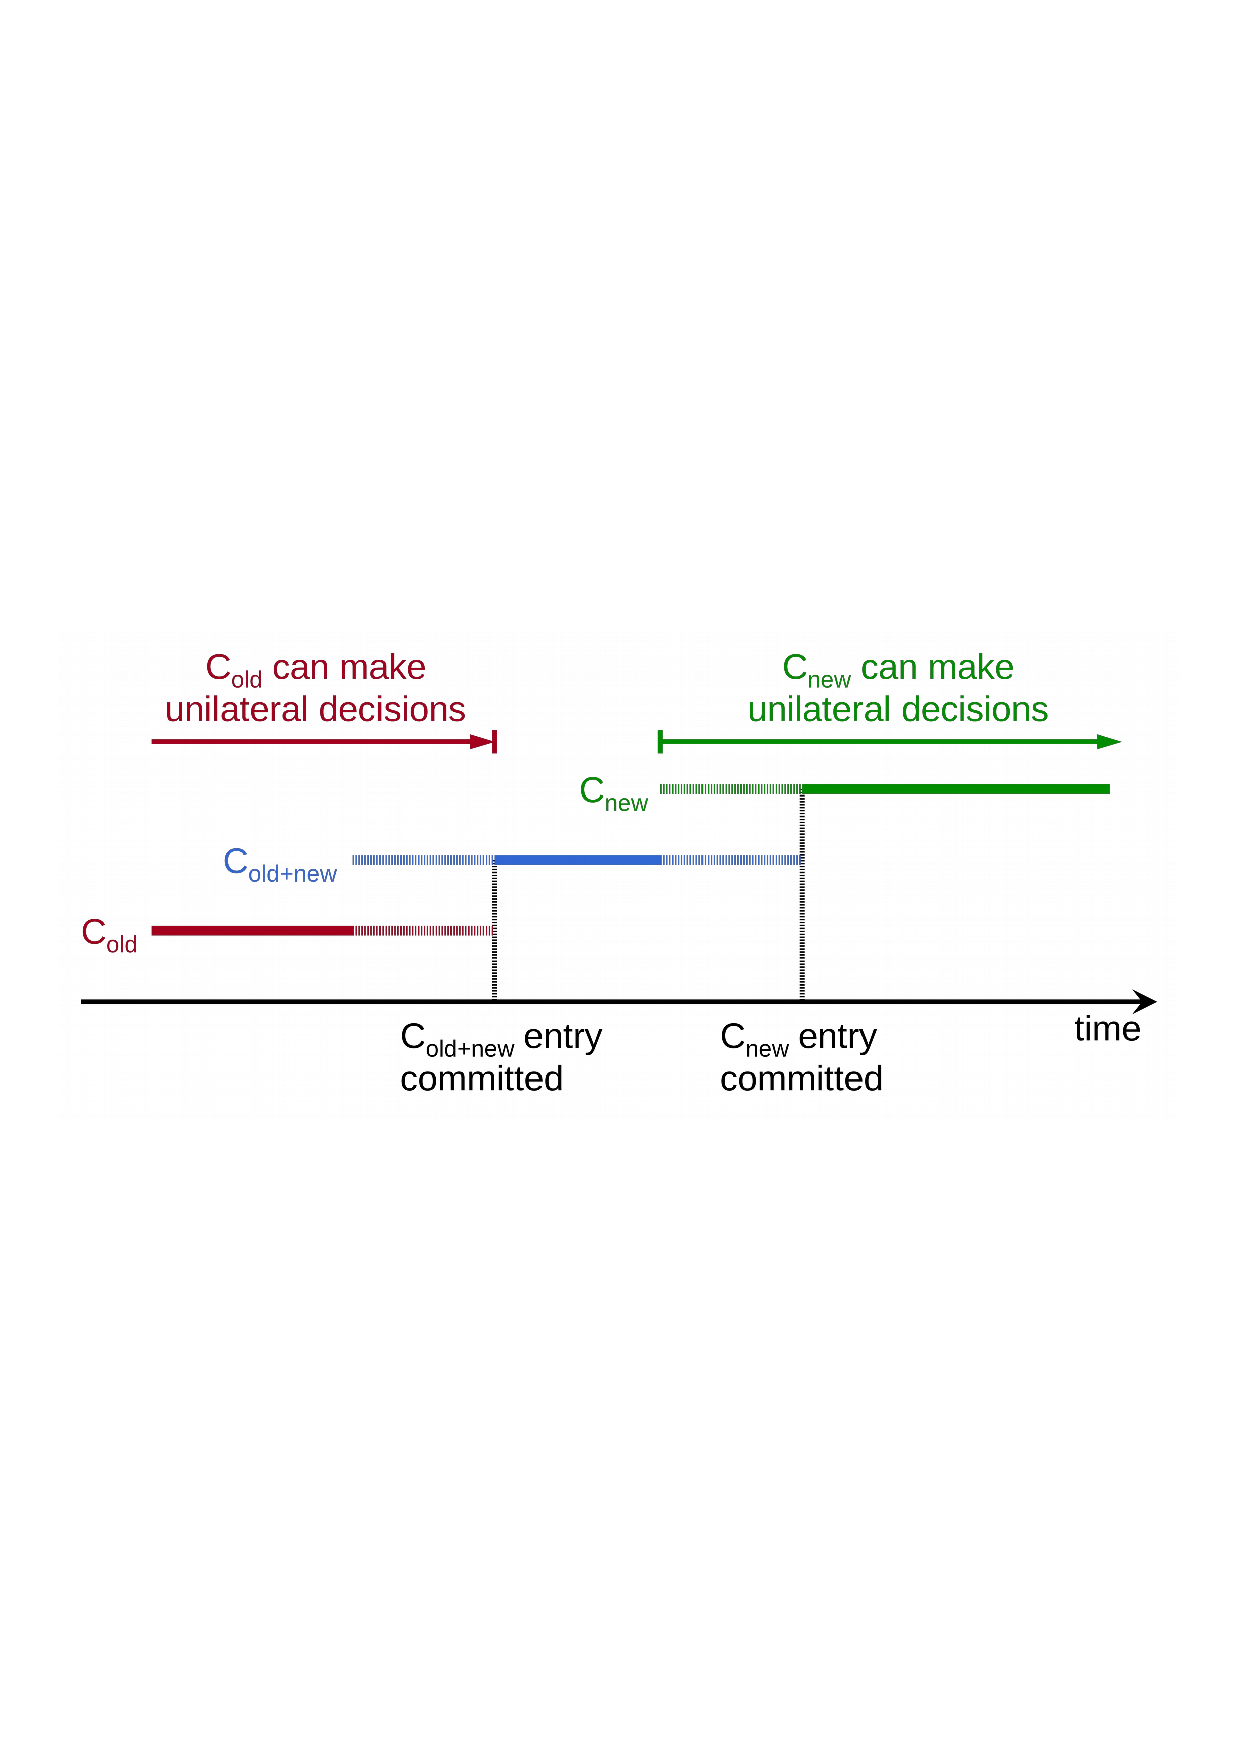
\includegraphics[width=0.90\columnwidth]{raft/jointConsensus.pdf}
    \caption{Linea temporale che mostra le fasi del passaggio del sistema da una configurazione all'altra.}
    \label{fig:figure 9}
  \end{figure}

